\documentclass[preprint,showkeys,nofootinbib]{revtex4-1}


% linking references
\usepackage{hyperref}
\hypersetup{
  breaklinks=true,
  colorlinks=true,
  linkcolor=blue,
  urlcolor=cyan,
}


% general physics / math packages and commands
\usepackage{physics,amsmath,amssymb,braket,dsfont}
\renewcommand{\t}{\text} % text in math mode
\newcommand{\f}{\dfrac} % shorthand for fractions
\newcommand{\p}[1]{\left(#1\right)} % parenthesis
\renewcommand{\sp}[1]{\left[#1\right]} % square parenthesis
\renewcommand{\set}[1]{\left\{#1\right\}} % curly parenthesis
\newcommand{\bk}{\braket} % shorthand for braket

\renewcommand{\d}{\text{d}}
\newcommand{\g}{\text{g}}
\newcommand{\e}{\text{e}}
\newcommand{\x}{\text{x}}
\newcommand{\y}{\text{y}}
\newcommand{\z}{\text{z}}

\renewcommand{\c}{\hat{c}}
\newcommand{\n}{\hat{n}}

\newcommand{\A}{\mathcal{A}}
\newcommand{\B}{\mathcal{B}}
\newcommand{\D}{\mathcal{D}}
\newcommand{\E}{\mathcal{E}}
\newcommand{\G}{\mathcal{G}}
\renewcommand{\H}{\mathcal{H}}
\newcommand{\I}{\mathcal{I}}
\newcommand{\K}{\mathcal{K}}
\renewcommand{\L}{\mathcal{L}}
\newcommand{\M}{\mathcal{M}}
\newcommand{\N}{\mathcal{N}}
\renewcommand{\O}{\mathcal{O}}
\renewcommand{\P}{\mathcal{P}}
\newcommand{\Q}{\mathcal{Q}}
\renewcommand{\S}{\mathcal{S}}
\newcommand{\U}{\mathcal{U}}

\newcommand{\1}{\mathds{1}}

\newcommand{\mA}{m_{\text{A}}} % symbol for the mass of an atom


% "left vector" arrow; requires tikz package
\newcommand{\lvec}[1]
{\reflectbox{\ensuremath{\vec{\reflectbox{\ensuremath{#1}}}}}}


% figures
\usepackage{graphicx} % for figures
\usepackage{grffile} % help latex properly identify figure extensions
\graphicspath{{./figures/}} % set path for all figures
\usepackage[caption=false]{subfig} % subfigures (via \subfloat[]{})


% inline lists
\usepackage[inline]{enumitem}


% for feynman diagrams
\usepackage{tikz,tikz-feynman}
\tikzset{
  baseline = (current bounding box.center)
}
\tikzfeynmanset{
  compat = 1.1.0,
  every feynman = {/tikzfeynman/small}
}
\newcommand{\shrink}[1]{\scalebox{0.8}{#1}} % for smaller diagrams


% color definitions (used in a figure)
\usepackage{xcolor}
\definecolor{lightblue}{RGB}{31,119,180}
\definecolor{orange}{RGB}{255,127,14}
\definecolor{green}{RGB}{44,160,44}
\definecolor{lightred}{RGB}{214,39,40}

% proper coloring inside math environment
\makeatletter
\def\mathcolor#1#{\@mathcolor{#1}}
\def\@mathcolor#1#2#3{
  \protect\leavevmode
  \begingroup
    \color#1{#2}#3
  \endgroup
}
\makeatother
\newcommand{\bmu}{\mathcolor{lightblue}{\mu}}
\newcommand{\onu}{\mathcolor{orange}{\nu}}
\newcommand{\grho}{\mathcolor{green}{\rho}}
\newcommand{\re}{\mathcolor{lightred}{\text{e}}}


% leave a note in the text, visible in the compiled document
\newcommand{\note}[1]{\textcolor{red}{#1}}

% for strikeout text
% normalem included to prevent underlining titles in the bibliography
\usepackage[normalem]{ulem}


\newcommand{\blue}[1]{\textcolor{blue}{#1}}
\newcommand{\red}[1]{\textcolor{red}{#1}}
\newcommand{\green}[1]{\textcolor{green}{#1}}


\begin{document}

\section*{Referee 1}

We thank the referee for taking the time to carefully read and
reconsider our revised manuscript.  Below, we address the remaining
comments made by the referee.

Excerpts from the referee reports are written in \blue{blue}, excerpts
from the previous version of our manuscript (i.e.~after the first
round of review) are written in \red{red}, and excerpts from the final
version of our manuscript is written in \green{green}.  All page,
line, equation, and reference numbers generally refer to those from
the previous version of our manuscript.


\begin{enumerate}
\item Concerning:

  \blue{The authors have significantly improved the manuscript and
    very carefully incorporated the comments in the first round of
    referee reports, and provided a very careful reply to each
    comment. The referee appreciates a lot this effort, and the
    manuscript can be published in the present form as it is.}

  We thank the referee for recognizing our efforts in the first round
  of referee reports, and for noting that we ``have significantly
  improved the manuscript'' to the point that it ``can be published in
  the present form''.


\item Concerning the remaining questions about renormalization:

  \blue{However, the referee as an optional comment, which the authors
    might consider. It concerns the renormalization and the question
    whether it is universal. The authors define the condition for
    renormalization in Eq.(16) by fixing the two-particle interaction
    in the lowest motional state. However, this procedure does not
    uniquely define the renormalization of the diagrams such as (23),
    where the loop is connected to an excited states. Especially, the
    authors claim that from Eq.(25) it follows Eq.~(26). However, the
    referee disagrees with this assessment as Eq (25) only fixes the
    counter term with all states in the motional ground
    state. However, the counter terms with excited external lines is
    not defined by this condition, and especially, there is no unique
    method to define it. Note, that this is in contrast to high energy
    physics, where the renormalization and form of the counter terms
    are uniquely fixed by Lorentz invariance and gauge
    symmetry. Therefore, the referee is convinced that the three-body
    interaction derived in the present manuscript also involves terms,
    which are non universal and involve additional contribution
    dependent on the strength of the optical lattice. The comparison
    between theory and experiment certainly is consistent with such an
    observation as the agreement is not exzellent.}

  We greatly thank the referee for their careful attention to detail.
  Indeed, our renormalization condition in Eq.~(16) (page 15) fixes
  counter-terms with all atoms in the lowest motional state, which at
  third order in the effective theory implies Eq.~(25) (page 19).
  While Eq.~(25) can be used to solve for counter-terms directly,
  factoring out any dependence on motional states, the referee is
  correct in pointing out that we have made an error in claiming that
  Eq.~(25) implies Eq.~(26).  Once this error is fixed, however, the
  counter-terms in question are uniquely defined, and can be used to
  cancel out the divergence from diagrams of the form in Eq.~(23).

  We have fixed the error in both the analytical work in section III
  and numerical results shown in section IV of our manuscript.  We
  emphasize in particular that the corrections to our numerical
  results (presented in figures 3, 4, and 5) are small enough as to be
  nearly imperceptible to the eye, and therefore do not affect any of
  the discussions or conclusions in our manuscript.

  To this end, we have replaced the following text:

  \red{To leading order in the coupling constants, the renormalization
    condition in (16) implies that
    \begin{align}
     \shrink{
       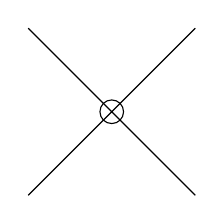
\begin{tikzpicture}
         \begin{feynman}
           \vertex[crossed dot] (v) {};
           \vertex[above left = of v] (f1);
           \vertex[below left = of v] (f2);
           \vertex[above right = of v] (f3);
           \vertex[below right = of v] (f4);
           \diagram* {
             (f1) -- (v),
             (f2) -- (v),
             (v) -- (f3),
             (v) -- (f4), };
         \end{feynman}
       \end{tikzpicture}}
     = \shrink{
       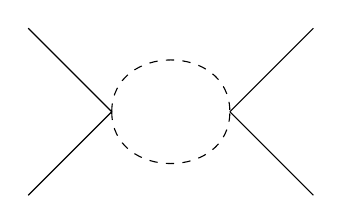
\begin{tikzpicture}
         \begin{feynman}
           \vertex (v1);
           \vertex[right = of v1] (v2);
           \vertex[above left = of v1] (f1);
           \vertex[below left = of v1] (f2);
           \vertex[above right = of v2] (f3);
           \vertex[below right = of v2] (f4);
           \diagram* {
             (f1) -- (v1) --[half left, scalar] (v2) -- (f3),
             (f2) -- (v1) --[half right, scalar] (v2) -- (f4), };
         \end{feynman}
       \end{tikzpicture}},
     \tag{25}
   \end{align}
   which means that the sum over all counter-term diagrams in (24) is
   \begin{align}
     \shrink{
       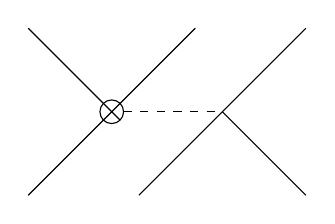
\begin{tikzpicture}
         \begin{feynman}
           \vertex[crossed dot] (v1) {};
           \vertex[right = 4em of v1] (v2);
           \vertex[above left = of v1] (f1);
           \vertex[below left = of v1] (f2);
           \vertex[above right = of v1] (f3);
           \vertex[below left = of v2] (f4);
           \vertex[below right = of v2] (f5);
           \vertex[above right = of v2] (f6);
           \diagram* {
             (f1) -- (v1) -- (f3),
             (f2) -- (v1) --[scalar] (v2),
             (f4) -- (v2) -- (f5),
             (v2) -- (f6), };
         \end{feynman}
       \end{tikzpicture}}
     = \shrink{
       \begin{tikzpicture}
         \begin{feynman}
           \vertex (v1);
           \vertex[right = of v1] (v2);
           \vertex[below right = of v2] (v3);
           \vertex[above left = of v1] (f1);
           \vertex[below left = of v1] (f2);
           \vertex[below left = of v3] (f3);
           \vertex[above right = of v2] (f4);
           \vertex[above right = of v3] (f5);
           \vertex[below right = of v3] (f6);
           \diagram* {
             (f1) -- (v1) --[half left, scalar] (v2) -- (f4),
             (f2) -- (v1) --[half right, scalar] (v2)
             --[scalar] (v3) -- (f5),
             (f3) -- (v3) -- (f6), };
         \end{feynman}
       \end{tikzpicture}}.
     \tag{26}
   \end{align}
   The net contribution of the these counter-term diagrams together
   with the two-particle-loop diagrams in (23) is therefore
   \begin{multline}
     - \shrink{
       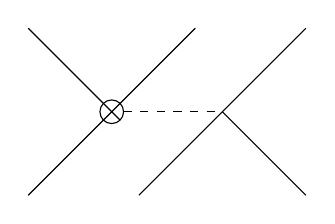
\begin{tikzpicture}
         \begin{feynman}
           \vertex[crossed dot] (v1) {};
           \vertex[right = 4em of v1] (v2);
           \vertex[above left = of v1] (f1);
           \vertex[below left = of v1] (f2);
           \vertex[above right = of v1] (f3);
           \vertex[below left = of v2] (f4);
           \vertex[below right = of v2] (f5);
           \vertex[above right = of v2] (f6);
           \diagram* {
             (f1) -- (v1) -- (f3),
             (f2) -- (v1) --[scalar] (v2),
             (f4) -- (v2) -- (f5),
             (v2) -- (f6), };
         \end{feynman}
       \end{tikzpicture}}
     + \shrink{
       \begin{tikzpicture}
         \begin{feynman}
           \vertex (v1);
           \vertex[right = of v1] (v2);
           \vertex[below right = of v2] (v3);
           \vertex[above left = of v1] (f1);
           \vertex[below left = of v1] (f2);
           \vertex[below left = of v3] (f3);
           \vertex[above right = of v2] (f4);
           \vertex[above right = of v3] (f5);
           \vertex[below right = of v3] (f6);
           \diagram* {
             (f1) -- (v1) --[half left, scalar] (v2) -- (f4),
             (f2) -- (v1) --[half right, scalar] (v2)
             --[scalar] (v3) -- (f5),
             (f3) -- (v3) -- (f6), };
         \end{feynman}
       \end{tikzpicture}}
     - \f12 \shrink{
       \begin{tikzpicture}
         \begin{feynman}
           \vertex (v1);
            \vertex[right = of v1] (v2);
            \vertex[below right = of v2] (v3);
            \vertex[above left = of v1] (f1);
            \vertex[below left = of v1] (f2);
            \vertex[below left = of v3] (f3);
            \vertex[above right = of v2] (f4);
            \vertex[above right = of v3] (f5);
            \vertex[below right = of v3] (f6);
            \diagram* {
              (f1) -- (v1) --[half left, scalar] (v2) -- (f4),
              (f2) -- (v1) --[half right, scalar] (v2)
              -- (v3) -- (f5),
              (f3) -- (v3) -- (f6), };
          \end{feynman}
        \end{tikzpicture}}
      - \f12 \shrink{
        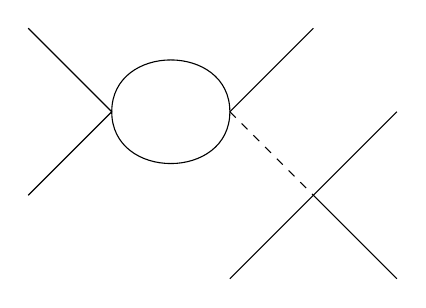
\begin{tikzpicture}
          \begin{feynman}
            \vertex (v1);
            \vertex[right = of v1] (v2);
            \vertex[below right = of v2] (v3);
            \vertex[above left = of v1] (f1);
            \vertex[below left = of v1] (f2);
            \vertex[below left = of v3] (f3);
            \vertex[above right = of v2] (f4);
            \vertex[above right = of v3] (f5);
            \vertex[below right = of v3] (f6);
            \diagram* {
              (f1) -- (v1) --[half left] (v2) -- (f4),
              (f2) -- (v1) --[half right] (v2)
              --[scalar] (v3) -- (f5),
              (f3) -- (v3) -- (f6), };
          \end{feynman}
        \end{tikzpicture}} \\
      = - \f12 \shrink{
        \begin{tikzpicture}
          \begin{feynman}
            \vertex (v1);
            \vertex[right = of v1] (v2);
            \vertex[below right = of v2] (v3);
            \vertex[above left = of v1] (f1);
            \vertex[below left = of v1] (f2);
            \vertex[below left = of v3] (f3);
            \vertex[above right = of v2] (f4);
            \vertex[above right = of v3] (f5);
            \vertex[below right = of v3] (f6);
            \diagram* {
              (f1) -- (v1) --[half left, scalar] (v2) -- (f4),
              (f2) -- (v1) --[half right, scalar] (v2)
              -- (v3) -- (f5),
              (f3) -- (v3) -- (f6), };
          \end{feynman}
        \end{tikzpicture}}
      - \f12 \shrink{
        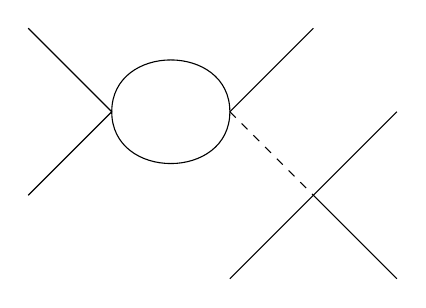
\begin{tikzpicture}
          \begin{feynman}
            \vertex (v1);
            \vertex[right = of v1] (v2);
            \vertex[below right = of v2] (v3);
            \vertex[above left = of v1] (f1);
            \vertex[below left = of v1] (f2);
            \vertex[below left = of v3] (f3);
            \vertex[above right = of v2] (f4);
            \vertex[above right = of v3] (f5);
            \vertex[below right = of v3] (f6);
            \diagram* {
              (f1) -- (v1) --[half left] (v2) -- (f4),
              (f2) -- (v1) --[half right] (v2)
              --[scalar] (v3) -- (f5),
              (f3) -- (v3) -- (f6), };
          \end{feynman}
        \end{tikzpicture}}.
      \tag{27}
    \end{multline}
    An identical cancellation occurs for the mirror images of the
    diagrams in (23) and (24), which results in a contribution to the
    effective Hamiltonian that is equal to (27).}

  by:

  \green{The sum over loop diagrams in (23), meanwhile, contains a
    divergence that must be cancelled out by the counter-terms in
    (24).  To leading order in the coupling constants, the
    renormalization condition in (16) implies that
    \begin{align}
      \shrink{
        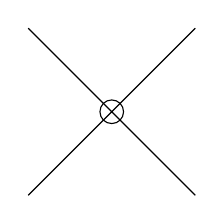
\begin{tikzpicture}
          \begin{feynman}
            \vertex[crossed dot] (v) {};
            \vertex[above left = of v] (f1);
            \vertex[below left = of v] (f2);
            \vertex[above right = of v] (f3);
            \vertex[below right = of v] (f4);
            \diagram* {
              (f1) -- (v),
              (f2) -- (v),
              (v) -- (f3),
              (v) -- (f4), };
          \end{feynman}
        \end{tikzpicture}}
      = \shrink{
        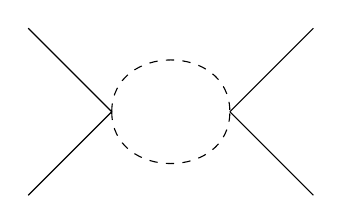
\begin{tikzpicture}
          \begin{feynman}
            \vertex (v1);
            \vertex[right = of v1] (v2);
            \vertex[above left = of v1] (f1);
            \vertex[below left = of v1] (f2);
            \vertex[above right = of v2] (f3);
            \vertex[below right = of v2] (f4);
            \diagram* {
              (f1) -- (v1) --[half left, scalar] (v2) -- (f3),
              (f2) -- (v1) --[half right, scalar] (v2) -- (f4), };
          \end{feynman}
        \end{tikzpicture}},
      \tag{30}
    \end{align}
    which can be expanded and solved explicitly for the counter-terms
    to find
    \begin{align}
      \widetilde G^{rs}_{r''s''}
      = \sum_{\ell,m,r',s'} \f{K_{\ell m}^2}{K E_{\ell m}}
      G^{rs}_{r's'} G^{r's'}_{r''s''}.
      \tag{31}
    \end{align}
    In terms of ordinary coupling constants, the counter-term diagram
    in (24) is therefore
    \begin{align}
      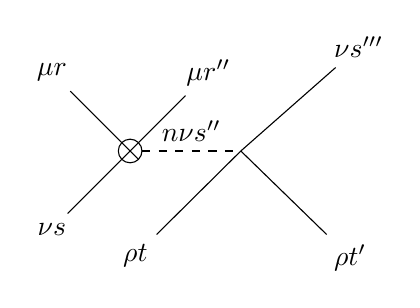
\begin{tikzpicture}
        \begin{feynman}
          \vertex[crossed dot] (v1) {};
          \vertex[above left = 4em of v1] (f1) {$\mu r$};
          \vertex[below left = 4em of v1] (f2) {$\nu s$};
          \vertex[right = 4em of v1] (v2);
          \vertex[above right = 4em of v1] (f3) {$\mu r''$};
          \vertex[below left = of v2] (f4) {$\rho t$};
          \vertex[below right = of v2] (f5) {$\rho t'$};
          \vertex[above right = of v2] (f6) {$\nu s'''$};
          \diagram* {
            (f1) -- (v1) -- (f3),
            (f2) -- (v1)
            --[scalar, edge label=$n\nu s''$] (v2),
            (f4) -- (v2) -- (f5),
            (v2) -- (f6), };
        \end{feynman}
      \end{tikzpicture}
      = \sum_{\ell,m,r',s'}
      \f{K_{\ell m}^2 K_n^2}{K E_{\ell m} E_n}
      G^{rs}_{r's'} G^{r's'}_{r''s''} G^{s''t}_{s'''t'}
      \c_{\mu r''}^\dag \c_{\nu s'''}^\dag \c_{\rho t'}^\dag
      \c_{\rho t} \c_{\nu s} \c_{\mu r}.
      \tag{32}
    \end{align}
    Altogether, the contribution to the third-order three-body
    interaction Hamiltonian from loop diagrams of the form in (23) and
    counter-term diagrams of the form in (24) is
    \begin{multline}
      \shrink{
        \begin{tikzpicture}
          \begin{feynman}
            \vertex (v1);
            \vertex[right = of v1] (v2);
            \vertex[below right = of v2] (v3);
            \vertex[above left = of v1] (f1);
            \vertex[below left = of v1] (f2);
            \vertex[below left = of v3] (f3);
            \vertex[above right = of v2] (f4);
            \vertex[above right = of v3] (f5);
            \vertex[below right = of v3] (f6);
            \diagram* {
              (f1) -- (v1) --[half left, scalar] (v2) -- (f4),
              (f2) -- (v1) --[half right, scalar] (v2)
              --[scalar] (v3) -- (f5),
              (f3) -- (v3) -- (f6), };
          \end{feynman}
        \end{tikzpicture}}
        - \shrink{
        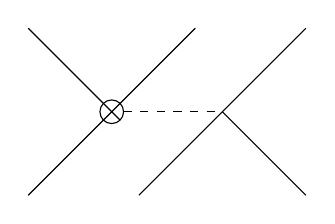
\begin{tikzpicture}
          \begin{feynman}
            \vertex[crossed dot] (v1) {};
            \vertex[right = 4em of v1] (v2);
            \vertex[above left = of v1] (f1);
            \vertex[below left = of v1] (f2);
            \vertex[above right = of v1] (f3);
            \vertex[below left = of v2] (f4);
            \vertex[below right = of v2] (f5);
            \vertex[above right = of v2] (f6);
            \diagram* {
              (f1) -- (v1) -- (f3),
              (f2) -- (v1) --[scalar] (v2),
              (f4) -- (v2) -- (f5),
              (v2) -- (f6), };
          \end{feynman}
        \end{tikzpicture}}
      - \f12 \shrink{
        \begin{tikzpicture}
          \begin{feynman}
            \vertex (v1);
            \vertex[right = of v1] (v2);
            \vertex[below right = of v2] (v3);
            \vertex[above left = of v1] (f1);
            \vertex[below left = of v1] (f2);
            \vertex[below left = of v3] (f3);
            \vertex[above right = of v2] (f4);
            \vertex[above right = of v3] (f5);
            \vertex[below right = of v3] (f6);
            \diagram* {
              (f1) -- (v1) --[half left, scalar] (v2) -- (f4),
              (f2) -- (v1) --[half right, scalar] (v2)
              -- (v3) -- (f5),
              (f3) -- (v3) -- (f6), };
          \end{feynman}
        \end{tikzpicture}}
      - \f12 \shrink{
        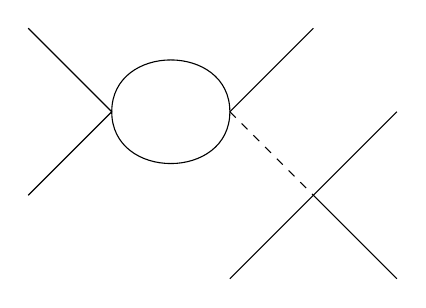
\begin{tikzpicture}
          \begin{feynman}
            \vertex (v1);
            \vertex[right = of v1] (v2);
            \vertex[below right = of v2] (v3);
            \vertex[above left = of v1] (f1);
            \vertex[below left = of v1] (f2);
            \vertex[below left = of v3] (f3);
            \vertex[above right = of v2] (f4);
            \vertex[above right = of v3] (f5);
            \vertex[below right = of v3] (f6);
            \diagram* {
              (f1) -- (v1) --[half left] (v2) -- (f4),
              (f2) -- (v1) --[half right] (v2)
              --[scalar] (v3) -- (f5),
              (f3) -- (v3) -- (f6), };
          \end{feynman}
        \end{tikzpicture}} \\
      = \p{\alpha_{3,2}^{(3)}
        - \f12\alpha_{4,3}^{(3)} - \f12\alpha_5^{(3)}}
      \H_{3,2}^{(3)},
      \tag{33}
    \end{multline}
    where
    \begin{align}
      \alpha_{3,2}^{(3)}
      \equiv \sum_{\substack{\ell+m>0\\n>0}}
      \f{K_{\ell m} K_n}{E_{\ell m} E_n}
      \p{K^{\ell m}_n - \f{K_{\ell m} K_n}{K}},
      &&
      \alpha_{4,3}^{(3)}
      \equiv K \sum_{m+n>0} \f{K_{mn}^2}{E_{mn}^2},
      \tag{34}
    \end{align}
    and
    \begin{align}
      \H_{3,2}^{(3)} \equiv \sum_{\abs{\set{\mu,\nu,\rho}}=3}
      G^{rs}_{r's'} G^{r's'}_{r''s''} G^{s''t}_{s'''t'}
      \c_{\mu r''}^\dag \c_{\nu s'''}^\dag \c_{\rho t'}^\dag
      \c_{\rho t} \c_{\nu s} \c_{\mu r}.
      \tag{35}
    \end{align}
    An equal contribution comes from the mirror images of these
    diagrams, such that the net third-order three-body interaction
    Hamiltonian is
    \begin{align}
      H_3^{(3)} = \p{\alpha_{3,1}^{(3)} - \alpha_5^{(3)}} \H_{3,1}^{(3)}
      + \p{2\alpha_{3,2}^{(3)} - \alpha_{4,3}^{(3)} - \alpha_5^{(3)}}
      \H_{3,2}^{(3)}.
      \tag{36}
    \end{align}
    Note that the aforementioned divergence and its cancellation are
    buried in $\alpha_{3,2}^{(3)}$.  Formally, this factor is
    calculated by imposing an ultraviolet cutoff $\Lambda$ for the
    maximum values of motional state indices $\ell,m,n$, and then
    taking the limit $\Lambda\to\infty$.  This procedure ensures that
    $\alpha_{3,2}^{(3)}$ always remains finite.}

  Accordingly, in the last appendix (G) we have replaced all instances
  of \red{$\alpha_3^{(1)}$} with \green{$\alpha_{3,1}^{(3)}$}, and the
  replaced prefactor \red{$-\p{\alpha_{4,3}^{(3)}+\alpha_5^{(3)}}$} by
  \green{$+ \p{2\alpha_{3,2}^{(3)} - \alpha_{4,3}^{(3)} -
      \alpha_5^{(3)}}$}.

  We have also re-organized the text in section III.D to improve
  readability in light of the above changes, and similarly
  re-organized the text in section III.E in order for this section to
  have a structure similar to that of section III.D.

  In full, sections III.D and III.E now read:

  \green{{\bf Effective three-body interactions at third order}}

  \green{The third-order effective interaction Hamiltonian
    $H_{\t{int}}^{(3)}$ in (14) contains both three- and four-body
    terms.  To compactly enumerate and evaluate all three-body
    diagrams at third order, we introduce an expanded coupling symbol
    \begin{align}
      G^{\mu q;\nu r}_{\rho s;\sigma t} \equiv \left\{
        \begin{array}{ll}
          G^{qr}_{st} & ~ \p{\mu,\nu} = \p{\rho,\sigma}
          \\
          - G^{qr}_{ts} & ~ \p{\mu,\nu} = \p{\sigma,\rho}
          \\
          0 & ~ \t{otherwise}
        \end{array}\right.
      \tag{20}
    \end{align}
    for more general
    $\p{\mu,q}+\p{\nu,r}\leftrightarrow\p{\rho,s}+\p{\sigma,t}$
    coupling induced by terms proportional to
    $\c_{\rho s}^\dag \c_{\sigma t}^\dag \c_{\nu r} \c_{\mu q}$.  The
    minus sign in (20) accounts for fermionic statistics: if
    $\p{\mu,\nu}=\p{\sigma,\rho}$, then we are considering a term of
    the form
    \begin{align}
      G^{\mu q;\nu r}_{\nu s;\mu t}
      \c_{\nu s}^\dag \c_{\mu t}^\dag \c_{\nu r} \c_{\mu q}
      = -G^{qr}_{ts} \c_{\nu s}^\dag \c_{\mu t}^\dag \c_{\mu r} \c_{\nu q}
      = G^{qr}_{ts} \c_{\mu t}^\dag \c_{\nu s}^\dag \c_{\nu r} \c_{\mu q}.
    \end{align}
    At the cost of introducing an additional sum over new nuclear spin
    indices, the expanded coupling symbol allows us to collect
    together diagrams which have the same graph topology, but
    represent different matrix elements of the effective Hamiltonian
    due to the exchange of nuclear spins at a vertex.  The third order
    three-body diagrams in $H_{\t{int}}^{(3)}$ are then
    \begin{align}
      \begin{tikzpicture}
        \begin{feynman}
          \vertex (v1);
          \vertex[below right = of v1] (v2);
          \vertex[above right = of v2] (v3);
          \vertex[above left = of v1] (f1) {$\mu r$};
          \vertex[left = of v1] (f2) {$\nu s$};
          \vertex[below left = of v2] (f3) {$\rho t$};
          \vertex[above right = of v3] (f4) {$\mu r''$};
          \vertex[right = of v3] (f5) {$\nu's'''$};
          \vertex[below right = of v2] (f6) {$\rho't'$};
          \diagram* {
            (f1) -- (v1) --[scalar, edge label=$\ell\mu r'$] (v3)
            -- (f4),
            (f2) -- (v1)
            --[scalar, edge label'=$m\nu s'$] (v2)
            --[scalar, edge label'=$n\nu's''$] (v3)
            -- (f5),
            (f3) -- (v2) -- (f6), };
        \end{feynman}
      \end{tikzpicture}
      \propto K_{\ell m} K^m_n K_{\ell n}
      G^{rs}_{r's'} G^{\nu s';\rho t}_{\nu's'';\rho't'} G^{r's''}_{r''s'''}
      \c_{\mu r''}^\dag \c_{\nu's'''}^\dag \c_{\rho't'}^\dag
      \c_{\rho t} \c_{\nu s} \c_{\mu r},
      \tag{22}
    \end{align}
    \begin{align}
      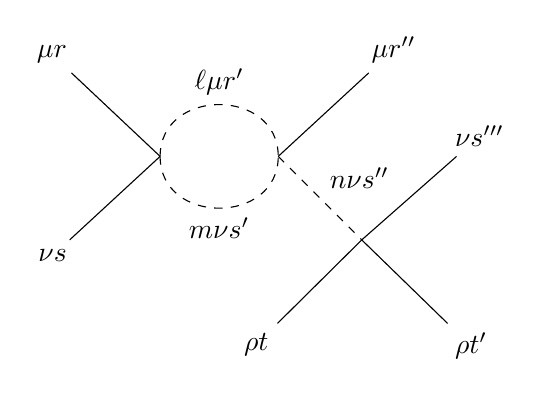
\begin{tikzpicture}
        \begin{feynman}
          \vertex (v1);
          \vertex[right = of v1] (v2);
          \vertex[below right = of v2] (v3);
          \vertex[above left = of v1] (f1) {$\mu r$};
          \vertex[below left = of v1] (f2) {$\nu s$};
          \vertex[below left = of v3] (f3) {$\rho t$};
          \vertex[above right = of v2] (f4) {$\mu r''$};
          \vertex[above right = of v3] (f5) {$\nu s'''$};
          \vertex[below right = of v3] (f6) {$\rho t'$};
          \diagram* {
            (f1) -- (v1)
            --[half left, scalar, edge label=$\ell\mu r'$] (v2)
            -- (f4),
            (f2) -- (v1)
            --[half right, scalar, edge label'=$m\nu s'$] (v2)
            --[scalar, edge label=$n\nu s''$] (v3)
            -- (f5),
            (f3) -- (v3) -- (f6), };
        \end{feynman}
      \end{tikzpicture}
      \propto K_{\ell m} K^{\ell m}_n K_n
      G^{rs}_{r's'} G^{r's'}_{r''s''} G^{s''t}_{s'''t'}
      \c_{\mu r''}^\dag \c_{\nu s'''}^\dag \c_{\rho t'}^\dag
      \c_{\rho t} \c_{\nu s} \c_{\mu r},
      \tag{23}
    \end{align}
    and the mirror image of (23).  As prescribed by
    $H_{\t{int}}^{(3)}$ in (14), these diagrams have an associated
    minus sign if they contain only one excited virtual state, and a
    factor of $1/2$ if they contain a virtual ground state.
    Remembering that counter-terms are $\O\p{G^2}$, there are
    additionally two third-order three-body diagrams in
    $H_{\t{int}}^{(2)}$, namely
    \begin{align}
      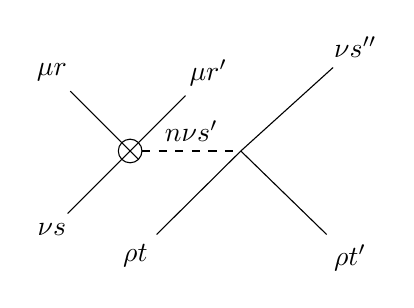
\begin{tikzpicture}
        \begin{feynman}
          \vertex[crossed dot] (v1) {};
          \vertex[above left = 4em of v1] (f1) {$\mu r$};
          \vertex[below left = 4em of v1] (f2) {$\nu s$};
          \vertex[right = 4em of v1] (v2);
          \vertex[above right = 4em of v1] (f3) {$\mu r'$};
          \vertex[below left = of v2] (f4) {$\rho t$};
          \vertex[below right = of v2] (f5) {$\rho t'$};
          \vertex[above right = of v2] (f6) {$\nu s''$};
          \diagram* {
            (f1) -- (v1) -- (f3),
            (f2) -- (v1)
            --[scalar, edge label=$n\nu s'$] (v2),
            (f4) -- (v2) -- (f5),
            (v2) -- (f6), };
        \end{feynman}
      \end{tikzpicture}
      \propto K_n^2 \widetilde G^{rs}_{r's'} G^{s't}_{s''t'}
      \c_{\mu r'}^\dag \c_{\nu s''}^\dag \c_{\rho t'}^\dag
      \c_{\rho t} \c_{\nu s} \c_{\mu r}
      \tag{24}
    \end{align}
    and its mirror image, where $\widetilde G^{qr}_{st}$ is equal to
    the counter-term associated with $G^{qr}_{st}$.}

  \green{The net contribution to the third-order three-body
    interaction Hamiltonian from three-particle-loop diagrams of the
    form in (22) is
    \begin{align}
     \shrink{
       \begin{tikzpicture}
         \begin{feynman}
           \vertex (v1);
           \vertex[below right = of v1] (v2);
           \vertex[above right = of v2] (v3);
           \vertex[above left = of v1] (f1);
           \vertex[left = of v1] (f2);
           \vertex[below left = of v2] (f3);
           \vertex[above right = of v3] (f4);
           \vertex[right = of v3] (f5);
           \vertex[below right = of v2] (f6);
           \diagram* {
             (f1) -- (v1) --[scalar] (v3) -- (f4),
             (f2) -- (v1) --[scalar] (v2) --[scalar] (v3) -- (f5),
             (f3) -- (v2) -- (f6), };
         \end{feynman}
       \end{tikzpicture}}
      - \f12 \shrink{
        \begin{tikzpicture}
          \begin{feynman}
            \vertex (v1);
            \vertex[below right = of v1] (v2);
            \vertex[above right = of v2] (v3);
            \vertex[above left = of v1] (f1);
            \vertex[left = of v1] (f2);
            \vertex[below left = of v2] (f3);
            \vertex[above right = of v3] (f4);
            \vertex[right = of v3] (f5);
            \vertex[below right = of v2] (f6);
            \diagram* {
              (f1) -- (v1) -- (v3) -- (f4),
              (f2) -- (v1) --[scalar] (v2) -- (v3) -- (f5),
              (f3) -- (v2) -- (f6), };
          \end{feynman}
        \end{tikzpicture}}
      - \f12 \shrink{
        \begin{tikzpicture}
          \begin{feynman}
            \vertex (v1);
            \vertex[below right = of v1] (v2);
            \vertex[above right = of v2] (v3);
            \vertex[above left = of v1] (f1);
            \vertex[left = of v1] (f2);
            \vertex[below left = of v2] (f3);
            \vertex[above right = of v3] (f4);
            \vertex[right = of v3] (f5);
            \vertex[below right = of v2] (f6);
            \diagram* {
              (f1) -- (v1) -- (v3) -- (f4),
              (f2) -- (v1) -- (v2) --[scalar] (v3) -- (f5),
              (f3) -- (v2) -- (f6), };
          \end{feynman}
        \end{tikzpicture}}
      = \p{\alpha_{3,1}^{(3)} - \alpha_5^{(3)}} \H_{3,1}^{(3)},
      \tag{25}
    \end{align}
    where
    \begin{align}
      \alpha_{3,1}^{(3)} \equiv \sum_{\substack{\ell+m>0\\\ell+n>0}}
      \f{K_{\ell m} K^m_n K_{\ell n}}{E_{\ell m} E_{\ell n}},
      &&
      \alpha_5^{(3)}
      \equiv  K \sum_{n>0} \f{K_n^2}{E_n^2},
      \tag{26}
    \end{align}
    and
    \begin{align}
      \H_{3,1}^{(3)} \equiv \sum_{\abs{\set{\mu,\nu,\rho}}=3}
      G^{rs}_{r's'} G^{\nu s'\rho t}_{\nu's''\rho't'} G^{r's''}_{r''s'''}
      \c_{\mu r''}^\dag \c_{\nu's'''}^\dag \c_{\rho't'}^\dag
      \c_{\rho t} \c_{\nu s} \c_{\mu r}.
      \tag{27}
    \end{align}
    Even though this contribution comes from loop diagrams, the
    factors $\alpha_{3,1}^{(3)}$ and $\alpha_5^{(3)}$ in (26) are
    finite.  At large motional state indices $n$, atoms become free
    particles for which $n$ essentially indexes discrete momentum
    states.  These atoms thus have an energy which asymptotically
    scales as $E_n\sim n^2\equiv n_\x^2+n_\y^2+n_\z^2$.  Furthermore,
    the oscillatory behavior of atomic wavefunctions with increasing
    motional state indices $\ell,m$ implies that the overlap integral
    $K_{\ell m}$ becomes sharply peaked at $\ell\approx m$ as $\ell$
    and $m$ get large.  The asymptotic behavior of
    $\alpha_{3,1}^{(3)}$ at large $\ell,m,n$ is therefore
    \begin{align}
      \alpha_{3,1}^{(3)}
      \sim \int \f{\d^3\ell~\d^3m~\d^3n}{\p{\ell^2+m^2}\p{\ell^2+n^2}}
      ~\delta\p{\ell-m}\delta\p{\ell-n}
      \sim \int \f{\d^3\ell}{\ell^4}
      \sim \int_{\ell_{\t{min}}}^\infty \f{\d\ell}{\ell^2}
      \sim \f1{\ell_{\t{min}}},
      \tag{28}
    \end{align}
    where in the last integral we changed to spherical coordinates,
    and $\ell_{\t{min}}^2$ is the minimum value of $\ell^2$ for which
    \begin{enumerate*}
    \item the energy $E_\ell\sim\ell^2$, and
    \item the integral expression in (28) is a good approximation to
      the corresponding sum in (26).
    \end{enumerate*}
    Note that the introduction of $\ell_{\t{min}}$ amounts to
    neglecting a finite number of terms in the sum over $\ell,m,n$ in
    (25), whose contribution to the value of $\alpha_{3,1}^{(3)}$ is
    finite.  Convergence of $\alpha_5^{(3)}$ is similarly guaranteed
    by the fact that the overlap integral $K_n$ does not
    asymptotically grow with increasing $n$, such that
    $\alpha_5^{(3)}$ asymptotically behaves as
    \begin{align}
      \alpha_5^{(3)} \sim \int \f{\d^3 n}{n^4}
      \sim \int_{n_{\t{min}}}^\infty \f{\d n}{n^2}
      \sim \f1{n_{\t{min}}},
      \tag{29}
    \end{align}
    where again $n_{\t{min}}$ is defined similarly to
    $\ell_{\t{min}}$.}

  \green{The sum over loop diagrams in (23), meanwhile, contains a
    divergence that must be cancelled out by the counter-terms in
    (24).  To leading order in the coupling constants, the
    renormalization condition in (16) implies that
    \begin{align}
      \shrink{
        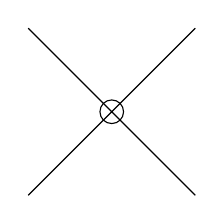
\begin{tikzpicture}
          \begin{feynman}
            \vertex[crossed dot] (v) {};
            \vertex[above left = of v] (f1);
            \vertex[below left = of v] (f2);
            \vertex[above right = of v] (f3);
            \vertex[below right = of v] (f4);
            \diagram* {
              (f1) -- (v),
              (f2) -- (v),
              (v) -- (f3),
              (v) -- (f4), };
          \end{feynman}
        \end{tikzpicture}}
      = \shrink{
        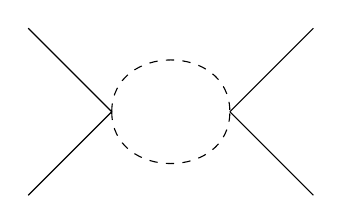
\begin{tikzpicture}
          \begin{feynman}
            \vertex (v1);
            \vertex[right = of v1] (v2);
            \vertex[above left = of v1] (f1);
            \vertex[below left = of v1] (f2);
            \vertex[above right = of v2] (f3);
            \vertex[below right = of v2] (f4);
            \diagram* {
              (f1) -- (v1) --[half left, scalar] (v2) -- (f3),
              (f2) -- (v1) --[half right, scalar] (v2) -- (f4), };
          \end{feynman}
        \end{tikzpicture}},
      \tag{30}
    \end{align}
    which can be expanded and solved explicitly for the counter-terms
    to find
    \begin{align}
      \widetilde G^{rs}_{r''s''}
      = \sum_{\ell,m,r',s'} \f{K_{\ell m}^2}{K E_{\ell m}}
      G^{rs}_{r's'} G^{r's'}_{r''s''}.
      \tag{31}
    \end{align}
    In terms of ordinary coupling constants, the counter-term diagram
    in (24) is therefore
    \begin{align}
      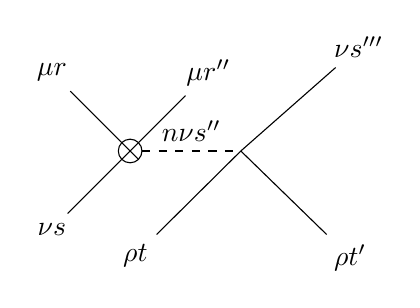
\begin{tikzpicture}
        \begin{feynman}
          \vertex[crossed dot] (v1) {};
          \vertex[above left = 4em of v1] (f1) {$\mu r$};
          \vertex[below left = 4em of v1] (f2) {$\nu s$};
          \vertex[right = 4em of v1] (v2);
          \vertex[above right = 4em of v1] (f3) {$\mu r''$};
          \vertex[below left = of v2] (f4) {$\rho t$};
          \vertex[below right = of v2] (f5) {$\rho t'$};
          \vertex[above right = of v2] (f6) {$\nu s'''$};
          \diagram* {
            (f1) -- (v1) -- (f3),
            (f2) -- (v1)
            --[scalar, edge label=$n\nu s''$] (v2),
            (f4) -- (v2) -- (f5),
            (v2) -- (f6), };
        \end{feynman}
      \end{tikzpicture}
      = \sum_{\ell,m,r',s'}
      \f{K_{\ell m}^2 K_n^2}{K E_{\ell m} E_n}
      G^{rs}_{r's'} G^{r's'}_{r''s''} G^{s''t}_{s'''t'}
      \c_{\mu r''}^\dag \c_{\nu s'''}^\dag \c_{\rho t'}^\dag
      \c_{\rho t} \c_{\nu s} \c_{\mu r}.
      \tag{32}
    \end{align}
    Altogether, the contribution to the third-order three-body
    interaction Hamiltonian from loop diagrams of the form in (23) and
    counter-term diagrams of the form in (24) is
    \begin{multline}
      \shrink{
        \begin{tikzpicture}
          \begin{feynman}
            \vertex (v1);
            \vertex[right = of v1] (v2);
            \vertex[below right = of v2] (v3);
            \vertex[above left = of v1] (f1);
            \vertex[below left = of v1] (f2);
            \vertex[below left = of v3] (f3);
            \vertex[above right = of v2] (f4);
            \vertex[above right = of v3] (f5);
            \vertex[below right = of v3] (f6);
            \diagram* {
              (f1) -- (v1) --[half left, scalar] (v2) -- (f4),
              (f2) -- (v1) --[half right, scalar] (v2)
              --[scalar] (v3) -- (f5),
              (f3) -- (v3) -- (f6), };
          \end{feynman}
        \end{tikzpicture}}
        - \shrink{
        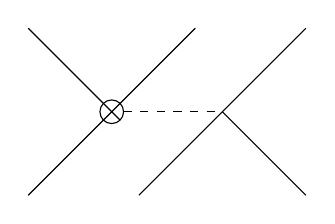
\begin{tikzpicture}
          \begin{feynman}
            \vertex[crossed dot] (v1) {};
            \vertex[right = 4em of v1] (v2);
            \vertex[above left = of v1] (f1);
            \vertex[below left = of v1] (f2);
            \vertex[above right = of v1] (f3);
            \vertex[below left = of v2] (f4);
            \vertex[below right = of v2] (f5);
            \vertex[above right = of v2] (f6);
            \diagram* {
              (f1) -- (v1) -- (f3),
              (f2) -- (v1) --[scalar] (v2),
              (f4) -- (v2) -- (f5),
              (v2) -- (f6), };
          \end{feynman}
        \end{tikzpicture}}
      - \f12 \shrink{
        \begin{tikzpicture}
          \begin{feynman}
            \vertex (v1);
            \vertex[right = of v1] (v2);
            \vertex[below right = of v2] (v3);
            \vertex[above left = of v1] (f1);
            \vertex[below left = of v1] (f2);
            \vertex[below left = of v3] (f3);
            \vertex[above right = of v2] (f4);
            \vertex[above right = of v3] (f5);
            \vertex[below right = of v3] (f6);
            \diagram* {
              (f1) -- (v1) --[half left, scalar] (v2) -- (f4),
              (f2) -- (v1) --[half right, scalar] (v2)
              -- (v3) -- (f5),
              (f3) -- (v3) -- (f6), };
          \end{feynman}
        \end{tikzpicture}}
      - \f12 \shrink{
        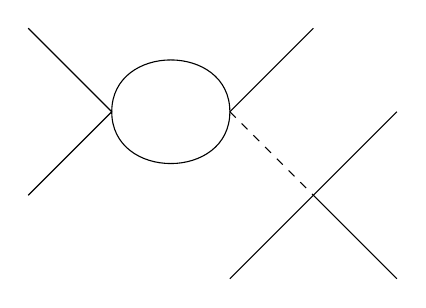
\begin{tikzpicture}
          \begin{feynman}
            \vertex (v1);
            \vertex[right = of v1] (v2);
            \vertex[below right = of v2] (v3);
            \vertex[above left = of v1] (f1);
            \vertex[below left = of v1] (f2);
            \vertex[below left = of v3] (f3);
            \vertex[above right = of v2] (f4);
            \vertex[above right = of v3] (f5);
            \vertex[below right = of v3] (f6);
            \diagram* {
              (f1) -- (v1) --[half left] (v2) -- (f4),
              (f2) -- (v1) --[half right] (v2)
              --[scalar] (v3) -- (f5),
              (f3) -- (v3) -- (f6), };
          \end{feynman}
        \end{tikzpicture}} \\
      = \p{\alpha_{3,2}^{(3)}
        - \f12\alpha_{4,3}^{(3)} - \f12\alpha_5^{(3)}}
      \H_{3,2}^{(3)},
      \tag{33}
    \end{multline}
    where
    \begin{align}
      \alpha_{3,2}^{(3)}
      \equiv \sum_{\substack{\ell+m>0\\n>0}}
      \f{K_{\ell m} K_n}{E_{\ell m} E_n}
      \p{K^{\ell m}_n - \f{K_{\ell m} K_n}{K}},
      &&
      \alpha_{4,3}^{(3)}
      \equiv K \sum_{m+n>0} \f{K_{mn}^2}{E_{mn}^2},
      \tag{34}
    \end{align}
    and
    \begin{align}
      \H_{3,2}^{(3)} \equiv \sum_{\abs{\set{\mu,\nu,\rho}}=3}
      G^{rs}_{r's'} G^{r's'}_{r''s''} G^{s''t}_{s'''t'}
      \c_{\mu r''}^\dag \c_{\nu s'''}^\dag \c_{\rho t'}^\dag
      \c_{\rho t} \c_{\nu s} \c_{\mu r}.
      \tag{35}
    \end{align}
    An equal contribution comes from the mirror images of these
    diagrams, such that the net third-order three-body interaction
    Hamiltonian is
    \begin{align}
      H_3^{(3)} = \p{\alpha_{3,1}^{(3)} - \alpha_5^{(3)}} \H_{3,1}^{(3)}
      + \p{2\alpha_{3,2}^{(3)} - \alpha_{4,3}^{(3)} - \alpha_5^{(3)}}
      \H_{3,2}^{(3)}.
      \tag{36}
    \end{align}
    Note that the aforementioned divergence and its cancellation are
    buried in $\alpha_{3,2}^{(3)}$.  Formally, this factor is
    calculated by imposing an ultraviolet cutoff $\Lambda$ for the
    maximum values of motional state indices $\ell,m,n$, and then
    taking the limit $\Lambda\to\infty$.  This procedure ensures that
    $\alpha_{3,2}^{(3)}$ always remains finite.}

  \green{{\bf Effective four-body interactions at third order}}

  \green{At third order in the coupling constants, we have four-body
    terms of the form
    \begin{align}
      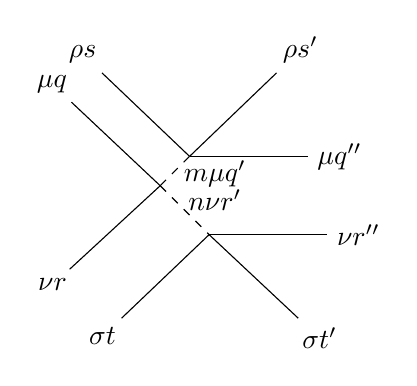
\begin{tikzpicture}
        \begin{feynman}
          \vertex (v1);
          \vertex[above right = 1.5em of v1] (v2);
          \vertex[below right = 2.5em of v1] (v3);
          \vertex[right = 0.5em of v1] (label)
          {$\let\scriptstyle\textstyle\substack{m\mu q'\\n\nu r'}$};
          \vertex[above left = of v1] (f1) {$\mu q$};
          \vertex[below left = of v1] (f2) {$\nu r$};
          \vertex[above left = of v2] (f3) {$\rho s$};
          \vertex[below left = of v3] (f4) {$\sigma t$};
          \vertex[above right = of v2] (f5) {$\rho s'$};
          \vertex[right = of v2] (f6) {$\mu q''$};
          \vertex[right = of v3] (f7) {$\nu r''$};
          \vertex[below right = of v3] (f8) {$\sigma t'$};
          \diagram* {
            (f1) -- (v1) --[scalar] (v2) -- (f6),
            (f2) -- (v1) --[scalar] (v3) -- (f7),
            (f3) -- (v2) -- (f5),
            (f4) -- (v3) -- (f8),
          };
        \end{feynman}
      \end{tikzpicture}
      \propto K_{mn} K_m K_n G^{qr}_{q'r'} G^{q's}_{q''s'} G^{r't}_{r''t'}
      \c_{\mu q''}^\dag \c_{\nu r''}^\dag
      \c_{\rho s'}^\dag \c_{\sigma t'}^\dag
      \c_{\sigma t} \c_{\rho s} \c_{\nu r} \c_{\mu q}
      \tag{37}
    \end{align}
    and its mirror image, as well as
    \begin{align}
      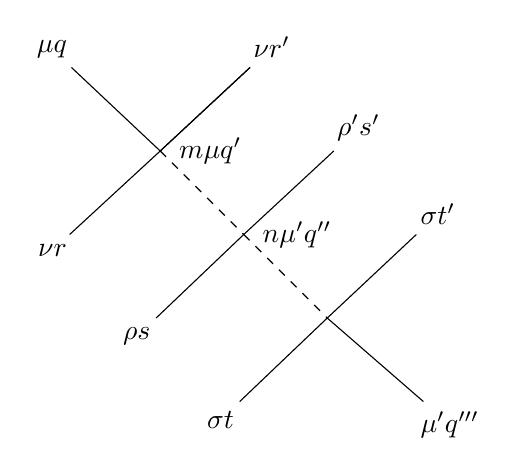
\begin{tikzpicture}
        \begin{feynman}
          \vertex[label=0:$~m\mu q'$] (v1);
          \vertex[below right = of v1, label=0:$~n\mu'q''$] (v2);
          \vertex[below right = of v2] (v3);
          \vertex[above left = of v1] (f1) {$\mu q$};
          \vertex[below left = of v1] (f2) {$\nu r$};
          \vertex[below left = of v2] (f3) {$\rho s$};
          \vertex[below left = of v3] (f4) {$\sigma t$};
          \vertex[above right = of v1] (f5) {$\nu r'$};
          \vertex[above right = of v2] (f6) {$\rho's'$};
          \vertex[above right = of v3] (f7) {$\sigma t'$};
          \vertex[below right = of v3] (f8) {$\mu'q'''$};
          \diagram* {
            (f1) -- (v1) -- (f5),
            (f2) -- (v1) -- (f5),
            (v1) --[scalar] (v2) --[scalar] (v3) -- (f8),
            (f3) -- (v2) -- (f6),
            (f4) -- (v3) -- (f7),
          };
        \end{feynman}
      \end{tikzpicture}
      \propto K_m K^m_n K_n
      G^{qr}_{q'r'} G^{\mu q'\rho s}_{\mu'q''\rho's'} G^{q''t}_{q'''t'}
      \c_{\mu'q'''}^\dag \c_{\nu r'}^\dag
      \c_{\rho's'}^\dag \c_{\sigma t'}^\dag
      \c_{\sigma t} \c_{\rho s} \c_{\nu r} \c_{\mu q}.
      \tag{38}
    \end{align}
    As we are computing the leading-order contribution to effective
    four-body interactions, there are no counter-terms contributions.
    In principle, there is now also the possibility to make the
    disconnected diagrams of the form
    \begin{align}
      \shrink{
        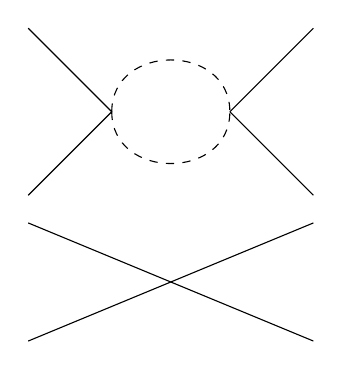
\begin{tikzpicture}
          \begin{feynman}
            \vertex (v1);
            \vertex[above left = of v1] (f1);
            \vertex[below left = of v1] (f2);
            \vertex[right = of v1] (v2);
            \vertex[above right = of v2] (f3);
            \vertex[below right = of v2] (f4);
            \vertex[below = 1em of f2] (f5);
            \vertex[below = of f5] (f6);
            \vertex[below = 1em of f4] (f7);
            \vertex[below = of f7] (f8);
            \diagram* {
              (f1) -- (v1),
              (f2) -- (v1),
              (v2) -- (f3),
              (v2) -- (f4),
              (v1) --[scalar, half left] (v2),
              (v1) --[scalar, half right] (v2),
              (f5) -- (f8),
              (f6) -- (f7) };
          \end{feynman}
        \end{tikzpicture}},
      &&
      \shrink{
        \begin{tikzpicture}
          \begin{feynman}
            \vertex (v1);
            \vertex[above left = of v1] (f1);
            \vertex[below left = of v1] (f2);
            \vertex[right = of v1] (v2);
            \vertex[above right = of v2] (f3);
            \vertex[below right = of v2] (f4);
            \vertex[left = of f2] (a1);
            \vertex[left = of f4] (a2);
            \vertex[below = 1em of a1] (f5);
            \vertex[below = of f5] (f6);
            \vertex[below = 1em of a2] (f7);
            \vertex[below = of f7] (f8);
            \diagram* {
              (f1) -- (v1),
              (f2) -- (v1),
              (v2) -- (f3),
              (v2) -- (f4),
              (v1) --[scalar, half left] (v2),
              (v1) --[scalar, half right] (v2),
              (f5) -- (f8),
              (f6) -- (f7) };
          \end{feynman}
        \end{tikzpicture}},
      &&
      \t{and}
      &&
      \shrink{
        \begin{tikzpicture}
          \begin{feynman}
            \vertex (v1);
            \vertex[above left = of v1] (f1);
            \vertex[below left = of v1] (f2);
            \vertex[right = of v1] (v2);
            \vertex[above right = of v2] (f3);
            \vertex[below right = of v2] (f4);
            \vertex[right = of f2] (a1);
            \vertex[right = of f4] (a2);
            \vertex[below = 1em of a1] (f5);
            \vertex[below = of f5] (f6);
            \vertex[below = 1em of a2] (f7);
            \vertex[below = of f7] (f8);
            \diagram* {
              (f1) -- (v1),
              (f2) -- (v1),
              (v2) -- (f3),
              (v2) -- (f4),
              (v1) --[scalar, half left] (v2),
              (v1) --[scalar, half right] (v2),
              (f5) -- (f8),
              (f6) -- (f7) };
          \end{feynman}
        \end{tikzpicture}}.
      \tag{39}
    \end{align}
    As prescribed by $H_{\t{int}}^{(3)}$ in (14), however, the second
    and third of these diagrams pick up a factor of $-1/2$, so the sum
    over disconnected diagrams vanishes.}

  \green{The contribution to the third-order four-body interaction
    Hamiltonian from diagrams of the form in (37) is
    \begin{align}
      \shrink{
        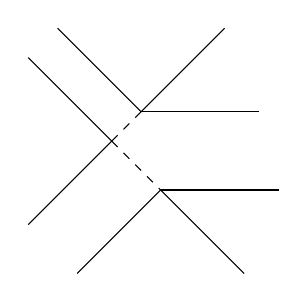
\begin{tikzpicture}
          \begin{feynman}
            \vertex (v1);
            \vertex[above right = 1.5em of v1] (v2);
            \vertex[below right = 2.5em of v1] (v3);
            \vertex[above left = of v1] (f1);
            \vertex[below left = of v1] (f2);
            \vertex[above left = of v2] (f3);
            \vertex[below left = of v3] (f4);
            \vertex[above right = of v2] (f5);
            \vertex[right = of v2] (f6);
            \vertex[right = of v3] (f7);
            \vertex[below right = of v3] (f8);
            \diagram* {
              (f1) -- (v1) --[scalar] (v2) -- (f6),
              (f2) -- (v1) --[scalar] (v3) -- (f7),
              (f3) -- (v2) -- (f5),
              (f4) -- (v3) -- (f8),
            };
          \end{feynman}
        \end{tikzpicture}}
      - \f12 \shrink{
        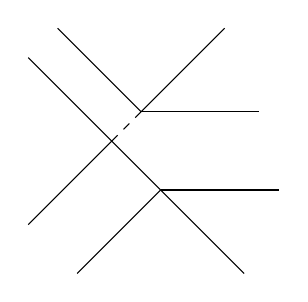
\begin{tikzpicture}
          \begin{feynman}
            \vertex (v1);
            \vertex[above right = 1.5em of v1] (v2);
            \vertex[below right = 2.5em of v1] (v3);
            \vertex[above left = of v1] (f1);
            \vertex[below left = of v1] (f2);
            \vertex[above left = of v2] (f3);
            \vertex[below left = of v3] (f4);
            \vertex[above right = of v2] (f5);
            \vertex[right = of v2] (f6);
            \vertex[right = of v3] (f7);
            \vertex[below right = of v3] (f8);
            \diagram* {
              (f1) -- (v1) --[scalar] (v2) -- (f6),
              (f2) -- (v1) -- (v3) -- (f7),
              (f3) -- (v2) -- (f5),
              (f4) -- (v3) -- (f8),
            };
          \end{feynman}
        \end{tikzpicture}}
      = \p{\alpha_{4,1}^{(3)} - \f12\alpha_5^{(3)}} \H_{4,1},
      \tag{40}
    \end{align}
    where
    \begin{align}
      \alpha_{4,1}^{(3)}
      \equiv \sum_{\substack{m\ge0\\n>0}} \f{K_{mn} K_m K_n}{E_{mn} E_n},
      \tag{41}
    \end{align}
    and
    \begin{align}
      \H_{4,1}^{(3)}
      \equiv \sum_{\abs{\set{\mu,\nu,\rho,\sigma}}=4}
      G^{qr}_{q'r'} G^{q's}_{q''s'} G^{r't}_{r''t'}
      \c_{\mu q''}^\dag \c_{\nu r''}^\dag
      \c_{\rho s'}^\dag \c_{\sigma t'}^\dag
      \c_{\sigma t} \c_{\rho s} \c_{\nu r} \c_{\mu q}.
      \tag{42}
    \end{align}
    An equal contribution comes from the mirror images of these
    diagrams.  The contribution from diagrams of the form in (38),
    meanwhile, is
    \begin{align}
      \shrink{
        \begin{tikzpicture}
          \begin{feynman}
            \vertex (v1);
            \vertex[below right = of v1] (v2);
            \vertex[below right = of v2] (v3);
            \vertex[above left = of v1] (f1);
            \vertex[below left = of v1] (f2);
            \vertex[below left = of v2] (f3);
            \vertex[below left = of v3] (f4);
            \vertex[above right = of v1] (f5);
            \vertex[above right = of v2] (f6);
            \vertex[above right = of v3] (f7);
            \vertex[below right = of v3] (f8);
            \diagram* {
              (f1) -- (v1) -- (f5),
              (f2) -- (v1) -- (f5),
              (v1) --[scalar] (v2) --[scalar] (v3) -- (f8),
              (f3) -- (v2) -- (f6),
              (f4) -- (v3) -- (f7),
            };
          \end{feynman}
        \end{tikzpicture}}
      - \f12 \shrink{
        \begin{tikzpicture}
          \begin{feynman}
            \vertex (v1);
            \vertex[below right = of v1] (v2);
            \vertex[below right = of v2] (v3);
            \vertex[above left = of v1] (f1);
            \vertex[below left = of v1] (f2);
            \vertex[below left = of v2] (f3);
            \vertex[below left = of v3] (f4);
            \vertex[above right = of v1] (f5);
            \vertex[above right = of v2] (f6);
            \vertex[above right = of v3] (f7);
            \vertex[below right = of v3] (f8);
            \diagram* {
              (f1) -- (v1) -- (f5),
              (f2) -- (v1) -- (f5),
              (v1) --[scalar] (v2) -- (v3) -- (f8),
              (f3) -- (v2) -- (f6),
              (f4) -- (v3) -- (f7),
            };
          \end{feynman}
        \end{tikzpicture}}
      - \f12 \shrink{
        \begin{tikzpicture}
          \begin{feynman}
            \vertex (v1);
            \vertex[below right = of v1] (v2);
            \vertex[below right = of v2] (v3);
            \vertex[above left = of v1] (f1);
            \vertex[below left = of v1] (f2);
            \vertex[below left = of v2] (f3);
            \vertex[below left = of v3] (f4);
            \vertex[above right = of v1] (f5);
            \vertex[above right = of v2] (f6);
            \vertex[above right = of v3] (f7);
            \vertex[below right = of v3] (f8);
            \diagram* {
              (f1) -- (v1) -- (f5),
              (f2) -- (v1) -- (f5),
              (v1) -- (v2) --[scalar] (v3) -- (f8),
              (f3) -- (v2) -- (f6),
              (f4) -- (v3) -- (f7),
            };
          \end{feynman}
        \end{tikzpicture}}
      = \p{\alpha_{4,2}^{(3)} - \alpha_5^{(3)}} \H_{4,2},
      \tag{43}
    \end{align}
    where
    \begin{align}
      \alpha_{4,2}^{(3)}
      \equiv \sum_{m,n>0} \f{K_m K^m_n K_n}{E_m E_n},
      \tag{44}
    \end{align}
    and
    \begin{align}
      \H_{4,2}^{(3)}
      \equiv \sum_{\abs{\set{\mu,\nu,\rho,\sigma}}=4}
      G^{qr}_{q'r'} G^{\mu q'\rho s}_{\mu'q''\rho's'} G^{q''t}_{q'''t'}
      \c_{\mu'q'''}^\dag \c_{\nu r'}^\dag
      \c_{\rho's'}^\dag \c_{\sigma t'}^\dag
      \c_{\sigma t} \c_{\rho s} \c_{\nu r} \c_{\mu q}.
      \tag{45}
    \end{align}
    The net third-order four-body interaction Hamiltonian is therefore
    \begin{align}
      H_4^{(3)}
      = \p{2\alpha_{4,1}^{(3)} - \alpha_5^{(3)}} \H_{4,1}^{(3)}
      + \p{\alpha_{4,2}^{(3)} - \alpha_5^{(3)}} \H_{4,2}^{(3)}.
      \tag{46}
    \end{align}}


\end{enumerate}

\end{document}
